% Pre-entrega del TP Especial - Redes de Información (ITBA, 2C 2026)
% Compilar: xelatex preentrega.tex  (dos veces, para el índice)
\documentclass[11pt,a4paper]{article}
\usepackage[margin=2.2cm]{geometry}
\usepackage{fontspec}
\setmainfont{Inter}[Scale=0.95]
\setmonofont{DejaVu Sans Mono}[Scale=0.82]
\usepackage[spanish,es-noquoting]{babel}
\usepackage{graphicx}
\usepackage{enumitem}
\usepackage{titlesec}
\usepackage{float}
\usepackage{caption}
\usepackage[hidelinks]{hyperref}
\usepackage{microtype}

\titleformat{\section}{\large\bfseries}{\thesection.}{0.6em}{}
\titlespacing*{\section}{0pt}{14pt}{6pt}
\setlist[itemize]{itemsep=2pt,topsep=4pt,leftmargin=1.4em}
\setlist[enumerate]{itemsep=6pt,topsep=4pt,leftmargin=1.6em}
\setlength{\parskip}{5pt}
\setlength{\emergencystretch}{2em}
\setlength{\parindent}{0pt}
\captionsetup{font=small}
\renewcommand{\contentsname}{\normalsize\bfseries Contenido}

\newcommand{\code}[1]{\texttt{#1}}

\begin{document}

% ---------------------------------------------------------------- Portada --
\begin{center}
\vspace*{2cm}
{\LARGE\bfseries Trabajo Práctico Especial - Redes}\\[6pt]
{\large ITBA - 2C 2026}\\[4pt]
{\large Gestión de Infraestructura por Código: Terraform}

\vspace{1.6cm}
{\bfseries Cátedra:}\\[4pt]
Santiago Raul Valles\\
Kevin Imanol Cortés Rodríguez\\
Juan Pablo Moreno\\
Alberto Ortega\\
Luis Alberto Staudenmann

\vspace{1.5cm}
{\bfseries Grupo NN:}\\[4pt]
Nombre Apellido, 00000\\
Nombre Apellido, 00000\\
Nombre Apellido, 00000
\end{center}

\vfill
\tableofcontents
\newpage

% ------------------------------------------------------------- Contenido --
\section{Contexto y Problemática}

Toda aplicación necesita, además de su código, una infraestructura sobre la cual ejecutarse:
redes con su direccionamiento, servidores, puntos de entrada, bases de datos y reglas de
filtrado. Cuando esa infraestructura se arma a mano, con clics en una consola o con una
secuencia de comandos, aparecen tres problemas conocidos: los entornos se vuelven
irrepetibles, porque cada servidor termina siendo un ejemplar único configurado de memoria
(lo que Fowler denominó \emph{snowflake server}); no queda registro de qué se cambió, cuándo
ni por qué; y la recuperación ante una falla depende de que alguien recuerde los pasos
exactos. Estas limitaciones son las que motivaron la aparición de las herramientas de
Infraestructura como Código (IaC), entre ellas Terraform.

The Store es una plataforma de comercio electrónico compuesta por cinco microservicios (UI,
Catalog, Cart, Orders y Checkout) escritos en distintos lenguajes (Java, Go y Node.js), cada
uno con su propio motor de persistencia. La cátedra la provee junto con un script de bash
(\code{local.sh}) que crea un clúster de Kubernetes local con kind, construye las imágenes de
los cinco servicios, las carga en el clúster y aplica un manifiesto YAML con todos los
objetos.

Ese script resuelve el arranque, pero arrastra las limitaciones propias de un enfoque
imperativo: describe una secuencia de pasos y no el resultado deseado. En concreto, no
mantiene registro de lo que existe, por lo que sólo sabe crear todo o borrarlo todo; no
detecta ni corrige las modificaciones hechas por fuera (si alguien altera el clúster con
\code{kubectl}, nadie se entera); no permite revisar por adelantado qué se va a modificar
antes de aplicar un cambio; y no contempla parametrizar el entorno (cantidad de nodos,
réplicas o versiones). Llevado a un entorno productivo el problema se agrava, porque habría
que crear además redes, subredes, clústeres, balanceadores y reglas de seguridad de forma
manual.

Se propone entonces adoptar Terraform para declarar como código toda la infraestructura que
The Store necesita, de manera versionable, auditable y reproducible.

\section{Diseño de la Solución}

Se utilizará Terraform (lenguaje HCL) para aprovisionar la totalidad del entorno, apoyándose
en cuatro providers oficiales: \code{docker} para la red y las imágenes, \code{kind} para el
clúster de Kubernetes, \code{kubernetes} para los objetos que corren dentro del clúster y
\code{helm} para instalar el controlador de Ingress.

El POC se despliega sobre un clúster local creado con kind (\emph{Kubernetes IN Docker}), la
misma plataforma que utiliza el script provisto por la cátedra. La decisión evita costos de
nube y dependencias externas durante la demostración, y mantiene a la vista toda la capa de
red (direccionamiento, NAT, ruteo entre nodos, resolución de nombres y reglas de filtrado),
que es precisamente lo que interesa analizar en esta materia y que un proveedor administrado
oculta detrás de su propia abstracción. El código se organiza de modo tal que migrar a una
nube implique reemplazar dos módulos (\code{networking} y \code{cluster}) sin tocar los otros
dos.

La infraestructura gestionada por Terraform se organiza en los siguientes módulos:

\begin{itemize}
  \item \textbf{Networking:} red \emph{bridge} de Docker con bloque 172.30.0.0/24 y su
    gateway, donde se conectan los nodos del clúster. Cumple el rol que en una nube cumpliría
    una VPC con sus subredes.
  \item \textbf{Cluster:} clúster de Kubernetes v1.35 con un nodo de control y dos nodos
    worker, con los bloques de direcciones de pods (10.244.0.0/16) y de servicios
    (10.96.0.0/16) declarados explícitamente, la publicación de los puertos 80 y 443 hacia la
    máquina anfitriona y la instalación del Ingress Controller (nginx), que actúa como
    balanceador de capa 7 y único punto de entrada. Equivale a un clúster administrado más su
    balanceador.
  \item \textbf{Databases:} las bases de datos de los microservicios que persisten
    información, MariaDB para Catalog, PostgreSQL para Orders y Redis para Checkout,
    desplegadas como StatefulSets con disco persistente. Las contraseñas las genera Terraform
    con el provider \code{random}, de modo que no hay credenciales escritas en el código.
    Equivalen a los servicios administrados de una nube (RDS y ElastiCache).
  \item \textbf{Application:} los cinco microservicios, cada uno con su Deployment (que
    mantiene N copias del proceso) y su Service (nombre DNS interno e IP virtual que balancea
    entre las copias); el Ingress que publica la tienda; y cuatro NetworkPolicies que
    segmentan el tráfico siguiendo el principio de mínimo privilegio, cumpliendo el rol de los
    \emph{security groups}.
\end{itemize}

La estructura de archivos será la siguiente:

\begin{quote}\small\ttfamily
terraform/\\
\hspace*{1em}main.tf\hfill\# Orquestación de los módulos y construcción de imágenes\\
\hspace*{1em}variables.tf\hfill\# Variables de entrada: nodos, réplicas, redes, versión\\
\hspace*{1em}outputs.tf\hfill\# Resultados: URL de la tienda, kubeconfig, bloques de red\\
\hspace*{1em}providers.tf\hfill\# docker, kind, kubernetes y helm\\
\hspace*{1em}terraform.tfvars\hfill\# Valores concretos del entorno\\
\hspace*{1em}modules/\\
\hspace*{2em}networking/\hfill\# Red y direccionamiento\\
\hspace*{2em}cluster/\hfill\# Clúster de Kubernetes e Ingress Controller\\
\hspace*{2em}databases/\hfill\# MariaDB, PostgreSQL y Redis\\
\hspace*{2em}application/\hfill\# Microservicios, Ingress y NetworkPolicies
\end{quote}

El estado de Terraform se mantiene en un archivo local, que ya provee bloqueo para evitar
ejecuciones concurrentes. Para el trabajo colaborativo del equipo se documenta la migración a
un backend remoto (bucket S3 con versionado y \emph{locking}, o Terraform Cloud), que implica
únicamente agregar un bloque \code{backend} sin modificar el resto del código.

\section{SCOPE del POC y casos de uso}

\textbf{Scope del proyecto:}

\begin{itemize}
  \item Provisionar la red del clúster con el bloque 172.30.0.0/24 y su gateway.
  \item Desplegar un clúster de Kubernetes v1.35 con un nodo de control y dos nodos worker,
    con los bloques de pods y servicios declarados en el código.
  \item Instalar el Ingress Controller y publicar la tienda en \code{http://the-store.localhost}.
  \item Construir las imágenes de los cinco microservicios a partir del código fuente provisto
    y cargarlas en los nodos del clúster.
  \item Desplegar los cinco microservicios y las tres bases de datos con disco persistente.
  \item Aplicar reglas de segmentación de red entre las capas de frontend, backend y datos.
  \item Demostrar el plan de ejecución (\code{terraform plan}) previo a cada cambio, la
    creación completa (\code{terraform apply}) y la destrucción completa
    (\code{terraform destroy}) del entorno.
  \item Demostrar modificaciones de infraestructura mediante los casos de uso descritos a
    continuación.
\end{itemize}

\textbf{Fuera de alcance:} despliegue en nube pública, integración continua, observabilidad,
gestión centralizada de logs, service mesh y certificados TLS, por corresponder a los temas de
otros grupos o no ser necesarios para demostrar el objetivo del trabajo.

\textbf{Casos de uso:}

\begin{enumerate}
  \item \textbf{Creación y destrucción completa del entorno de forma reproducible.} Se
    demuestra que toda la infraestructura puede crearse desde cero con \code{terraform apply}
    y eliminarse por completo con \code{terraform destroy}, sin residuos. Como complemento se
    demuestra la detección de \emph{drift}: se modifica un objeto a mano con \code{kubectl}
    (por ejemplo, se cambia la cantidad de réplicas o se borra un objeto), \code{terraform
    plan} detecta la diferencia entre el estado declarado y el real, y \code{terraform apply}
    la corrige. Es la capacidad que distingue a Terraform del script imperativo original.

  \item \textbf{Escalamiento ante un pico de demanda.} La tienda necesita absorber un volumen
    de tráfico mayor al habitual. Se modifica el archivo \code{terraform.tfvars} para aumentar
    las réplicas de los microservicios más solicitados (UI y Checkout) y, si hiciera falta más
    capacidad de cómputo, la cantidad de nodos worker del clúster. Se ejecuta \code{terraform
    plan} para verificar el alcance del cambio y luego \code{terraform apply}. Se demuestra
    que un cambio de configuración en un único archivo escala el entorno completo de forma
    controlada.

  \item \textbf{Actualización de versión y rollback.} Se descubre un problema en la versión
    desplegada de la aplicación. Se modifica la variable que define la versión de las
    imágenes, se aplica el cambio y Kubernetes ejecuta un \emph{rolling update} de los pods
    afectados sin interrumpir el servicio. Si la nueva versión introduce fallas, se revierte
    la variable al valor anterior y se vuelve a aplicar, demostrando la capacidad de volver
    atrás de forma controlada.

  \item \textbf{Respuesta a un incidente de seguridad.} Se detecta que un componente
    comprometido dentro del clúster intenta acceder directamente a la base de datos de
    órdenes. Se ajustan las NetworkPolicies declaradas en Terraform para restringir el acceso
    a la capa de datos únicamente desde los microservicios que la necesitan. Se ejecuta
    \code{terraform plan} para confirmar que sólo se modifican las reglas previstas y no el
    resto de la infraestructura, y se aplica el cambio. Se verifica el resultado comprobando
    que un pod ajeno a la aplicación ya no puede establecer conexión con la base.
\end{enumerate}

\section{Diagrama de Arquitectura}

El entorno completo corre sobre una máquina con Ubuntu 24.04 y Docker. Terraform crea una red
\emph{bridge} de Docker con el bloque \textbf{172.30.0.0/24} y gateway 172.30.0.1, que
funciona como un switch de capa 2 al que se conectan los nodos del clúster; el tráfico
saliente hacia Internet se enmascara con la dirección de la máquina anfitriona (SNAT).

Cada nodo del clúster es un contenedor Docker basado en Debian 12 que ejecuta \emph{containerd}
y \emph{kubelet}, y recibe una dirección de esa red: \textbf{172.30.0.2} el nodo de control y
\textbf{172.30.0.3} y \textbf{172.30.0.4} los dos nodos worker. Dentro del clúster se usan dos
bloques adicionales, disjuntos entre sí y respecto de la red de nodos y de la red local de la
máquina: \textbf{10.244.0.0/16} para las direcciones de los pods (cada nodo recibe un /24 de
ese bloque) y \textbf{10.96.0.0/16} para las direcciones virtuales de los Services, que
Kubernetes implementa con reglas de DNAT y que balancean el tráfico entre las copias de cada
microservicio. La resolución de nombres interna la provee CoreDNS en la dirección 10.96.0.10.

El nodo de control cumple además el rol de nodo de borde: es el único que publica puertos
hacia la máquina anfitriona (80 y 443) y sobre él corre el Ingress Controller. Un pedido del
navegador a \code{http://the-store.localhost} llega al puerto 80 del host, se reenvía por DNAT
al nodo de borde, el Ingress Controller lo enruta según la cabecera \code{Host} hacia el
Service de la UI, y éste lo entrega por DNAT a uno de los pods de UI en el puerto 8080. A
partir de ahí, la UI consulta por HTTP a los cuatro microservicios de backend usando sus
nombres DNS internos, y éstos consultan a sus bases de datos con los protocolos propios de
cada motor: MySQL sobre el puerto 3306, PostgreSQL sobre el 5432 y RESP sobre el 6379.

La segmentación se aplica con cuatro NetworkPolicies siguiendo el principio de mínimo
privilegio: por defecto ningún pod acepta conexiones entrantes; la UI sólo acepta tráfico
proveniente del Ingress Controller; los microservicios de backend sólo aceptan tráfico de la
UI y de otros backends; y las bases de datos sólo aceptan tráfico de los backends. Todos los
bloques utilizados son direcciones privadas y no se solapan entre sí.

\begin{figure}[H]
\centering
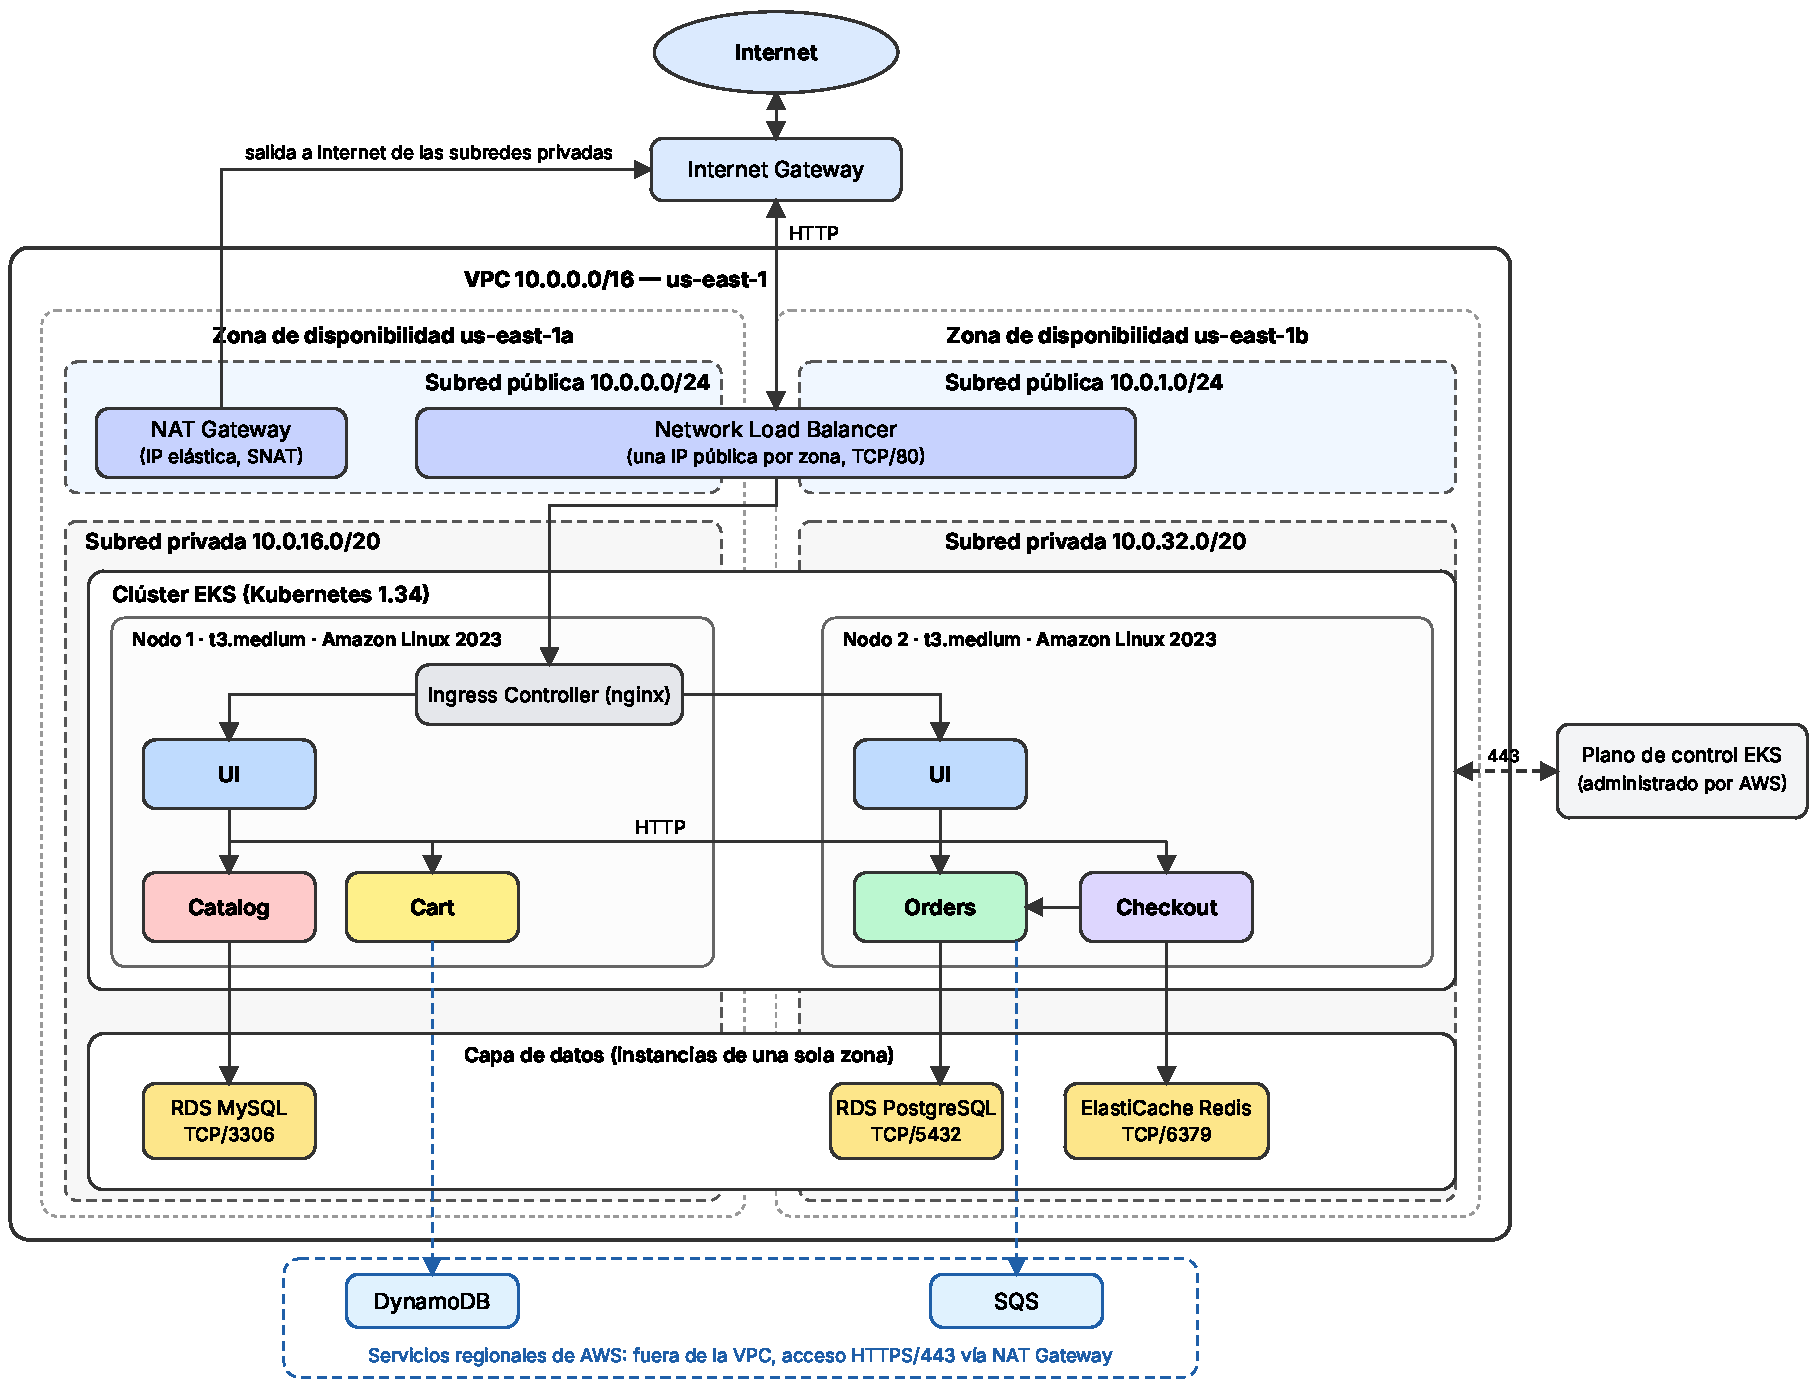
\includegraphics[width=\linewidth]{img/arquitectura.pdf}
\caption{Arquitectura del POC: bloques de direcciones, nodos, microservicios, bases de datos y
protocolos. En rojo el camino del tráfico del usuario; en negro el tráfico interno permitido
por las NetworkPolicies.}
\end{figure}

\section{Alternativas consideradas}

Como alternativa a \textbf{Terraform} se consideró \textbf{Pulumi}, que permite declarar
infraestructura con lenguajes de propósito general (TypeScript, Python, Go). Se optó por
Terraform porque HCL es un lenguaje declarativo diseñado específicamente para configuración de
infraestructura, lo que hace que el código sea más legible y que el plan de cambios sea
directo de revisar, y porque su ecosistema de providers y su documentación son más maduros.
También se evaluó \textbf{OpenTofu}, la bifurcación de código abierto de Terraform: es
compatible con el código escrito, pero se mantuvo Terraform por ser la herramienta nombrada en
el tema asignado.

Respecto de la plataforma, se consideró desplegar el POC sobre \textbf{una nube pública} (AWS,
con VPC, EKS, RDS y ElastiCache). Se descartó por tres motivos: implica un costo por hora
mientras el entorno está encendido, introduce una dependencia externa (credenciales, cuotas y
conectividad) durante una demostración que es remota, y oculta detrás de servicios
administrados buena parte de la capa de red que esta materia busca analizar. La estructura
modular elegida deja preparado ese camino: los módulos de aplicación y bases de datos son
independientes del proveedor.

Dentro de las opciones de Kubernetes local se evaluaron \textbf{minikube} y \textbf{k3d}.
minikube levanta por defecto un único nodo, lo que impediría mostrar el ruteo de tráfico entre
nodos; k3d utiliza k3s, una distribución reducida que incorpora su propio balanceador y
controlador de Ingress y por lo tanto esconde componentes que interesa mostrar. Se eligió kind
porque ejecuta Kubernetes sin modificaciones, permite declarar la topología y los bloques de
direcciones, y es la misma herramienta que emplea el script provisto por la cátedra.

Finalmente se consideró resolver el despliegue únicamente con \textbf{Helm} o con
\textbf{Ansible}. Helm y Kustomize sólo alcanzan a los objetos de Kubernetes: no crean la red,
el clúster ni las bases de datos. Ansible está orientado a la configuración de servidores y no
mantiene un estado con el que comparar la realidad, que es justamente la capacidad que se
quiere demostrar. De todos modos ambos enfoques son complementarios: en esta solución Helm se
invoca desde Terraform para instalar el Ingress Controller.

\section{Fuentes}

\begin{enumerate}[label={[\arabic*]}]
  \item HashiCorp. \emph{What is Terraform?} y \emph{The Core Terraform Workflow}.
    \url{https://developer.hashicorp.com/terraform/intro}
  \item Fowler, M. (2012). \emph{SnowflakeServer}. martinfowler.com.
    \url{https://martinfowler.com/bliki/SnowflakeServer.html}
  \item Morris, K. (2020). \emph{Infrastructure as Code: Dynamic Systems for the Cloud Age}
    (2\textsuperscript{a} ed.). O'Reilly Media.
  \item Kubernetes. \emph{Services, Load Balancing and Networking} y \emph{Network Policies}.
    \url{https://kubernetes.io/docs/concepts/services-networking/}
  \item kind. \emph{Quick Start} y \emph{Configuration}.
    \url{https://kind.sigs.k8s.io/docs/user/quick-start/}
  \item AWS Containers. \emph{Retail Store Sample Application}.
    \url{https://github.com/aws-containers/retail-store-sample-app}
\end{enumerate}

\end{document}
